\section{Preliminary Experiments}
\label{sec:experiment}

%% by comparing applying a model checker to original C language programs
%% with to abstracted behavior.

\subsection{Setup of the experiments}

We conducted preliminary experiments to check feasibility and to
investigate the problems in the current framework.  For the following
C programs, we extracted the behavioral types manually in the form of
another C programs.
\begin{itemize}
\item \texttt{poker.c}: A program that models a poker game.  It
  randomly deals cards to two players, compares the decks of the
  players, and decides the winner.
\item \texttt{database.c}: A program that models a database management
  system.  This program is taken from an online course of the C
  language~\cite{lch}.  The program allocates memory cells when it
  opens a database and deallocates the cells when it closes the
  database.
  %% It opens a database and performs some operations on the database
  %% (retrieve, delete and update data, or create a new database) and
  %% closes the database.  We rewrite this program as
  %% \texttt{database\_rw.c} without changing its meaning.  from website
  %% (http://c.learncodethehardway.org/book/ex17.html) by Zed Shaw,
  %% modeling a database.
\item \texttt{gen\_init\_cpio.c}: A module for a file system in the
  Linux kernel v.3.18.1.  It allocates a memory cell when it creates a
  file.  Deallocation is conducted in error-handling code.
\item \texttt{decompress\_unlzo.c}: A module in the Linux kernel
  v.3.18.1 that decompresses LZO files.  It allocates a memory cell to
  store the contents obtained from an input LZO file.  Deallocation
  occurs in error-handling code.
\end{itemize}

%% \begin{itemize}
%%   \item We rewrite this program as \texttt{poker\_rw.c} without
%%     changing its meaning.
%% \end{itemize}

For verifying that each program consumes only fixed amount of memory
cells, we applied CPAChecker~\cite{beyer2011cpachecker} (1) to the
original file and (2) to the file that represents the extracted
behavior.  All of the experiments are conducted on a machine with an
Intel(R) Core(TM) i7-3770 CPU @ 3.40GHz, 8MB cache and 3.76GB memory,
running on Debian (kernel version 2.6.32-5-amd64) and CPAchecker
(version 1.3.4).

%% We apply a model checker on these programs to check the property --
%% the number of memory usage does not exceed the number of available
%% memory cells.  In order to do it, in a program, we fixed a global
%% number $n$ which denotes the number of available memory for
%% allocation, it will decrease 1 when doing allocation and increase 1
%% when doing deallocation; we insert an assertion statement $assert(n
%% >= 0)$ after allocation statements. Hence, when doing model
%% checking on these programs, the checker will check if the property
%% is guaranteed.

\subsection{Result}

\begin{table}
  \scriptsize
\begin{tabular}{|c|c|c|c|c|c|c|}
\hline
& \multicolumn{6}{|c|}{\texttt{original programs}}  \\
\hline
& \texttt{loc} & \texttt{nfun} & \texttt{cpu time} & \texttt{memory (MB)} & \texttt{fixed num}& \texttt{verified result} \\
\hline
\texttt{poker.c} & 86 & 4 & 2.700 & 2797 & 4  & \texttt{TRUE}  \\
\hline
\texttt{database.c} & 153 & 10 & 12.010 & 2907 & 2  & \texttt{TRUE}  \\
\hline
\texttt{gen\_init\_cpio.c} & 346 & 19 & 9.580 & 2809 & 2  & \texttt{TRUE}  \\
\hline
\texttt{decompress\_unlzo.c} & 162 & 2  & 3.000  & 2806  & 2  & \texttt{TRUE}  \\
\hline
\end{tabular}
\caption{Result of the verification of the original C programs.}
\label{tb:mcc}
\end{table}

\begin{table}
  \scriptsize
\begin{tabular}{|c|c|c|c|c|c|c|}
\hline
&\multicolumn{6}{|c|}{abstracted behavior} \\
\hline
 &\texttt{loc} & \texttt{nfun} & \texttt{cpu time} & \texttt{memory (MB)} & \texttt{fixed num} & \texttt{verified result} \\
\hline
\texttt{poker.c} & 16 & 4 & 1.980 & 2803 & 4  & \texttt{FALSE}  \\
\hline
\texttt{database.c} &  16 & 4 & 2.060 & 2800 & 2 & \texttt{FALSE} \\
\hline
\texttt{gen\_init\_cpio.c} & 16 & 4 & 2.020 & 2802 & 2  & \texttt{FALSE}  \\
\hline
\texttt{decompress\_unlzo.c} & 16 & 4 & 1.970  & 2738  & 2  & \texttt{FALSE}  \\
\hline
\end{tabular}
\caption{Result of the verification of the extracted behavior.}
\label{tb:mca}
\end{table}

%% \begin{table}
%%   \scriptsize
%% \begin{tabular}{|c|c|c|c|c|c|c|}
%%   \hline
%% \texttt{poker\_rw.c} & 89 & 4 & 2.740 & 2800 & 4  & \texttt{TRUE}  \\
%% \hline
%% \texttt{database\_rw.c} & 151 & 10 & 7.080 & 2907 & 2  & \texttt{TRUE}  \\
%% \hline
%% \texttt{gen\_init\_cpio\_rw.c} & 343 &19  & 4.850  & 2744  & 2  & \texttt{TRUE}  \\
%% \hline
%% \texttt{decompress\_unlzo\_rw.c} & 92 & 2  & 2.650  & 2800  & 2  & \texttt{TRUE}  \\
%% \hline
%% \end{tabular}
%% \caption{Model checking on the original C programs.  (Rewritten.)}
%% \label{tb:mcarw}
%% \end{table}

%% \begin{table}
%%   \scriptsize
%% \begin{tabular}{|c|c|c|c|c|c|c|}
%%   \hline
%%   \texttt{poker\_rw.c} & 18 & 4 & 2.020 & 2798 & 4  & \texttt{TRUE}  \\
%%   \hline
%%   \texttt{database\_rw.c} &  18 & 4 & 1.990 & 2737 & 2 & \texttt{TRUE} \\
%%   \hline
%%   \texttt{gen\_init\_cpio\_rw.c} & 18 & 4 & 2.000  & 2742  & 2  & \texttt{TRUE}  \\
%%   \hline
%%   \texttt{decompress\_unlzo\_rw.c} & 18 & 4  & 2.000  & 2796  & 2  & \texttt{TRUE}  \\
%%   \hline
%% \end{tabular}
%% \caption{Model checking on an abstracted behavior}
%% \label{tb:mca}
%% \end{table}

Table~\ref{tb:mcc} and Table~\ref{tb:mca} show the result.  We present
the number of lines of each file (\texttt{loc}), the number of
functions (\texttt{nfun}), time spent by CPAChecker in seconds
(\texttt{cpu time}), the amount of memory in megabytes
(\texttt{memory}), the upper-bound of the number of consumed memory
cells (\texttt{fixed num}), and the result of the verification
(\texttt{verified result}).

\subsection{Discussion}

CPAChecker, when it is applied to the original programs, was able to
verify that the programs are totally memory-leak free.  However, the
verification failed for experiments with extracted behaviors.  This is
because our type system is not path-sensitive.  For example, a typical
pattern where verification with the extracted behaviors fail is as
follows.
\begin{verbatim}
while (...) {
  if (/* some condition c */) {
    x = malloc(sizeof(int));
  }
  /* Do something */
  if (/* condition equivalent to c */) {
    free(x);
  }
}
\end{verbatim}
For the program above, extracted behavior is \(\mu\alpha. (\mathbf{0}
+ \Malloc); (\mathbf{0} + \Free); \alpha\), which is not enough to
check no-memory-leak, although it is memory-leak free if the condition
\texttt{c} does not change between the allocation and the
deallocation.  Our type system can deal with the program above by
rewriting it to the following one.
\begin{verbatim}
while (...) {
  if (/* some condition c */) {
    x = malloc(sizeof(int));
    /* Do something */
    free(x);
  } else {
    /* Do something */
  }
}
\end{verbatim}
For the rewritten program, the extracted behavior is
\(\mu\alpha. ((\Malloc; \Free) + \mathbf{0}); \alpha\), for which the
predicate \(\OK_1\) holds.  We confirmed that CPAChecker can verify
\(\OK_1\) for the extracted behavior of the rewritten programs without
penalty on cpu time.

From the comparison of the Table~\ref{tb:mcc} and Table~\ref{tb:mca},
we can observe that the latter is more efficient than the former.

%% The column \texttt{original programs} and \texttt{abstracted behavior}
%% mean applying the model checker to a original C language program and
%% to abstracted behavior respectively.  These two columns consist of
%% several columns: $\sharp$\texttt{loc} means the number of program
%% locations; $\sharp$\texttt{fun} means the number of functions in a
%% program; \texttt{cpu time (total)} means the total execution time of
%% CPU in seconds; \texttt{memory(MB)} means the number of virtual memory
%% cells consumed by model checker in \texttt{MByte}; \texttt{fixed num}
%% means the number of available memory cells for allocation; the
%% \texttt{TRUE} in the \texttt{verified result} column means the number
%% of the memory cells which a program consumes does not exceed the
%% \texttt{fixed num}, otherwise it is \texttt{FALSE} which denotes
%% overflow.

%% The results present in the these two tables show that the
%% resources required for model checking become smaller if applying model
%% checkers to the abstracted behavior, since the abstracted behavior
%% only consists of allocation and deallocation.

%% One thing we should notice in these two tables is that for the same
%% programs, the \texttt{verified result} should be the same when model
%% checking on original programs and abstracted behavior; but it is not,
%% for example, \texttt{database.c} has the \texttt{TRUE} in the
%% Table~\ref{tb:mcc} but the \texttt{FALSE} in the
%% Table~\ref{tb:mca}. The reason is that our approach, abstracted
%% behavior, may not correctly deal with some conditional statements
%% about allocation and deallocation. For example, the behavior of
%% \texttt{database.c} is $\mu\alpha.\Malloc;\Malloc;(((\Free + 0);\Free)
%% + 0);\alpha)$, due to the choice type, it may perform like
%% $\mu\alpha.\Malloc;\Malloc;0;0;\alpha$, which means consuming unbound
%% number of memory cells. The rewritten \texttt{database\_rw.c}, which
%% does not change the semantics of original program, has the behavior
%% $\mu\alpha.(\Malloc;(\Malloc + \Free) + 0);\Free;\alpha)$ which
%% returns \texttt{TRUE} when doing model checking on it.


%% \begin{table}
%% \tiny
%% \begin{tabular}{|c|c|c|c|c|c|c|c|c|c|c|}
%% \hline
%% & \multicolumn{5}{|c|}{original programs} & \multicolumn{5}{|c|}{abstracted behavior} \\
%% \hline
%%  & $\sharp$loc & $\sharp$fun & cpu time (total) & memory (MB) & fixed num & $\sharp$loc & $\sharp$fun & cpu time (total) & memory (MB) & fixed num \\
%% \hline
%% linklist.c & 154 & 13 & 9.770 & 2943 & 6(true) & 20 & 4 & 3.190 & 2918 & 6(false) \\
%% \hline
%% linklst2.c & 140 & 13 & 25.620 & 2955 & 21(true) & 20 & 4 & 10.72 & 2945 & 21(false) \\
%% \hline
%% linkstack.c  & 87 & 10 & 10.830 & 2941 & 11(true) & 20 & 4 & 4.990 & 2916 & 11(false) \\
%% \hline
%% linkqueue.c & 119 & 11 & 13.110 & 2939 & 4(true) & 25 & 4 & 2.660 & 2919 & 4(false) \\
%% \hline
%% binarysorttree.c & 80 & 5 & 30.210 & 2950 & 10(true) & 19 & 4 & 5.130 & 2935 & 10(false) \\
%% \hline
%% database.c & 179 & 12 & 4.930 & 2922 & 3(true) & 21 & 4 & 2.760 & 2920 & 2(false) \\
%% \hline
%% ihex2fw.c & 202 & 7 & 23.490 & 2882 & 5(false) & 15 & 4 & 2.160 & 2797 & 5(false) \\
%% \hline
%% gen\_init\_cpio.c & 346 & 19 & 9.580 & 2809 & 1(true) & 15 & 4 & 2.160 & 2799 & 1(false) \\
%% \hline
%% \end{tabular}
%% %%\caption{My first table}
%% \end{table}

%% \begin{figure}
%%  \centering
%%  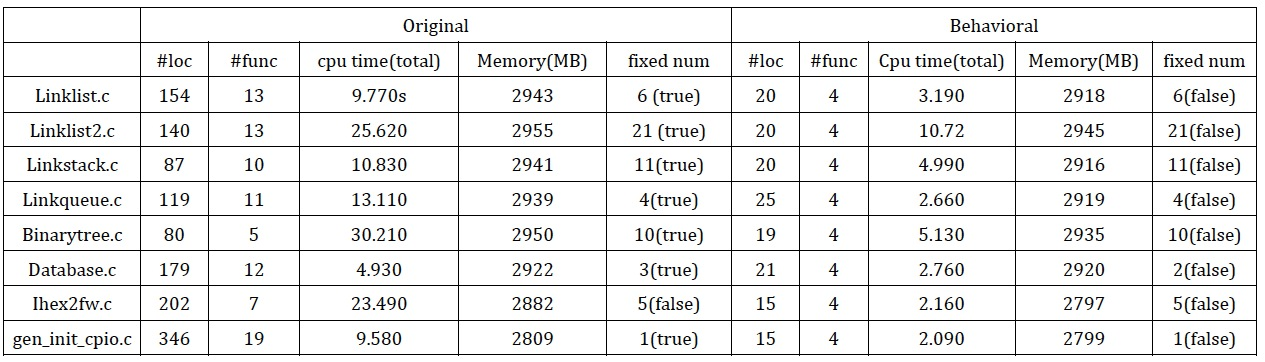
\includegraphics[width=14cm]{statistic.png}
%% \caption{Comparison}
%% \label{fig:statistic}
%% \end{figure}
